% Copyright 2007 by Till Tantau
%
% This file may be distributed and/or modified
%
% 1. under the LaTeX Project Public License and/or
% 2. under the GNU Public License.
%
% See the file doc/licenses/LICENSE for more details.


\lecture[25]{The least-squares line}{lecture-text}

\subtitle{and the correlation coefficient}

\date{3 December 2013}

% pp. 492-505


\begin{document}

\begin{frame}
  \maketitle
\end{frame}



\begin{frame}{Last time}
  \begin{enumerate}
      \item The \alert{correlation coefficient}, $r$,
      \item measures the strength of a linear relationship between two quantitative variables.
      \item It can be transformed to have a $t$ distribution
      \item under the null hypothesis of $r=0$ (no linear relationship).
  \end{enumerate}

    \vspace{2em}

    \structure{Today:} other ways to think about it.

\end{frame}

\begin{frame}\frametitle<presentation>{Outline}
  \tableofcontents
\end{frame}


\section{Prediction and line--fitting}


%%%%%%
\begin{frame}{Example:}
    Monthly mean minimum \& maximum temperatures
    at USC, 1906--2013  (1196 data points),
    \uncover<2->{with monthly means before 1920 subtracted}
    \begin{center}
    \includegraphics<1>{usc-temps.pdf}
    \includegraphics<2>{usc-temps-stdized.pdf}
    \end{center}

    \pause
    \vspace{2em}

    \begin{align*}
        r&=0.1582157 \\
        n&=1196 \\
        t_s &= r \sqrt{\frac{n-2}{1-r^2}} = 5.536772 
    \end{align*}
    and with $df=1194$, $P=3.79\times 10^{-8}$.

\end{frame}

\subsection{the SD line}

%%%%%%
\begin{frame}{Which line?}

    There are \structure{several reasons} to put a straight line through bivariate data:
    \begin{enumerate}
        \item visual emphasis
        \item quantitative description of the mean relationship (slope, intercept)
        \item prediction of $Y$ for new values of $X$
    \end{enumerate}


    \vspace{2em}

    \structure{Example:} interpolate temperatures for 1915--1920
    \begin{center}
    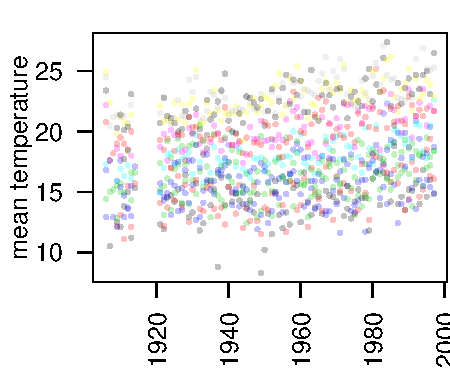
\includegraphics[width=.5\textwidth]{usc-temps.pdf}
    \end{center}

\end{frame}


%%%%%%
\begin{frame}{The SD line}

    One possible line is the \alert{SD line},
    that
    \begin{itemize}
        \item goes through the means $(\bar x, \bar y)$, and
        \item has slope $\pm s_x/s_y$.
    \end{itemize}
    (i.e.\ is $y=x$ on the plot of $z$-scores)

    \vspace{1em}

    \structure{Example:} \uncover<2->{with yearly means}

    \centering
    \includegraphics<1>{usc-temps-lines}
    \includegraphics<2>{usc-temps-lines-means}

\end{frame}

\subsection{the Regression Line}

%%%%%%
\begin{frame}{The line of Local Averages}

    \structure{Instead}, fit a model with a \alert{linear relationship between the means}:
    \begin{align*}
        Y &= \beta_0 + \beta_1 X + \epsilon, \\
        \text{so} \quad \mu_{Y|X} &= \beta_0 + \beta_1 X ,
    \end{align*}
    i.e.\ the mean value of $Y$ is linear in $X$.
    

    \begin{center}
        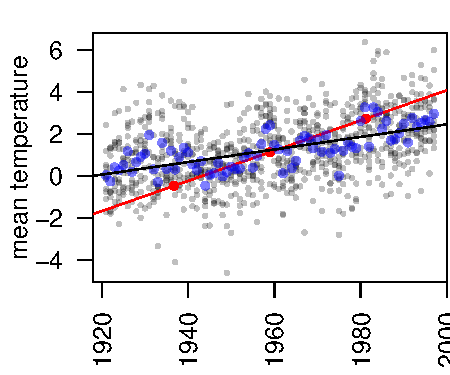
\includegraphics{usc-temps-both-lines}
    \end{center}

\end{frame}


%%%%%%
\begin{frame}{Relationship to $r$}

    The line of local averages,
    a.k.a.\ the \alert{regression line}
    has 
    \begin{align*}
        \text{(slope)}\quad b_1 &= r \; \frac{s_x}{s_y} \\
        \text{(intercept)}\quad b_0 &= \bar y - b_1 \bar x,
    \end{align*}
    i.e.\ slope $r$ in normalized coordinates,
    and passing through $(\bar x, \bar y)$.

    \vspace{2em}

    Our estimate of the mean of $Y$ given $X$ is then
    \[
        \hat \mu_{Y|X} = b_0 + b_1 X .
    \]

\end{frame}

%%%%%%
\begin{frame}{Example:}

    \centering
        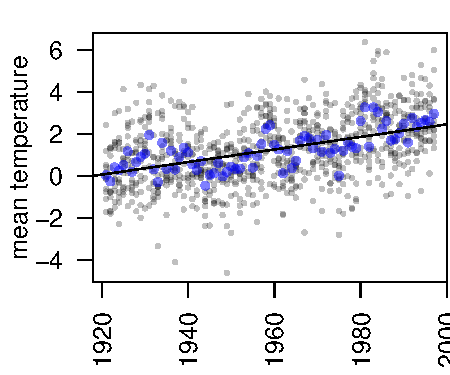
\includegraphics{usc-temps-regression}

    \begin{align*}
        \bar x &= 1966.917 & s_x &= 26.81045 \\
        \bar y &= 1.155366 & s_y &= 1.550648 \\
               r &= 0.3128291 & \hat \mu_{Y|X} &= 0.018 \; X - 33.8 .
    \end{align*}

\end{frame}

\section{Sums of squares}

\subsection{Residuals}


%%%%%%
\begin{frame}{Observed minus predicted}

    \begin{block}{Residuals}
        The residuals of a regression are the differences between the \structure{observed values} 
        and the \structure{predicted values},
        i.e.\ the vertical distances to the regression line,
        or the \alert{errors} we'd make if we predicted with the regression line.
    \end{block}

    \vspace{2em}

    Predicted:
    \[
        \hat y_i = b_0 + b_1 x_i
    \]
    Residual, or error:
    \[
        e_i = y_i - \hat y_i .
    \]

\end{frame}


%%%%%%
\begin{frame}{Residual sum of squares}

    \begin{block}{$\SS(\text{resid})$}
        The \alert{residual sum of squares} is the sum of the squares of the residuals:
        \[
            \SS(\text{resid}) = \sum_i (y_i - \hat y_i)^2 = \sum_i e_i^2 .
        \]
    \end{block}

    \vspace{2em}

    We are using the \structure{least squares regression line},\\
    which is the straight line that \alert{minimizes} $\SS(\text{resid})$.

    \vspace{2em}

    Amazing fact: the equation of this line is easy to compute,
    and is related to the correlation coefficient.


\end{frame}


%%%%%%
\begin{frame}{Residual SD}

    \begin{block}{$s_e$}
        The \alert{residual standard deviation} is
        \[ s_e = \sqrt{ \frac{ \sum (y_i - \hat y_i)^2 }{n-2} } = \sqrt{ \frac{ \SS(\text{resid}) }{ n-2 } } .  \]
    \end{block}

    \vspace{2em}

    This measures the spread of the points about the regression line.


\end{frame}


%%%%%%
\begin{frame}{Example:}
    \centering
        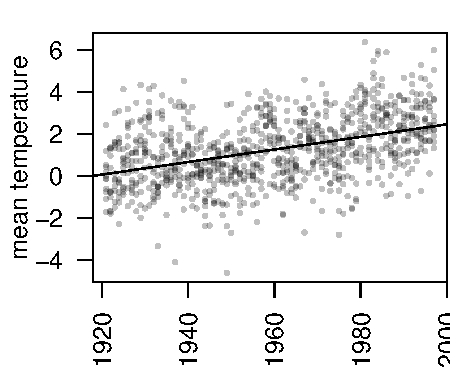
\includegraphics{usc-temps-just-regression}

    \begin{align*}
       r &= 0.3128291 \\
        s_e &= 2.110126 .
    \end{align*}


\end{frame}


%%%%%%
\begin{frame}{Partitioning sums of squares}

    Often, people report $r^2$ as the ``\alert{proportion of variance explained}'':
    \[
        r^2 = 1 - (1-\frac{1}{n-1}) \frac{s_e^2}{s_y^2} \approx 1 - \frac{s_e^2}{s_y^2}.
    \]

    \pause

    \only<1-2>{
\centering
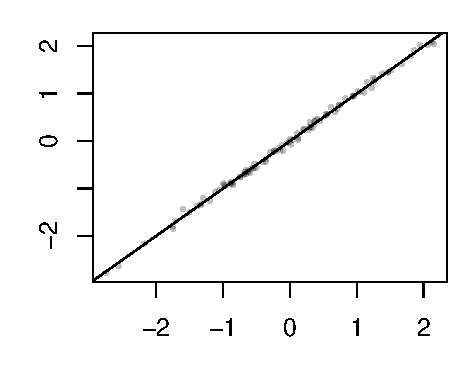
\includegraphics[height=2in]{r2ex-1.pdf}
        \[ r^2 = 0.9975455 \]
    }

    \only<3>{
\centering
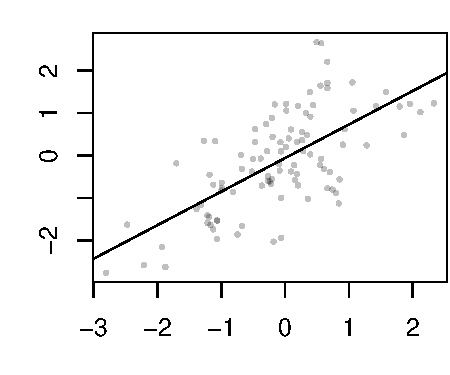
\includegraphics[height=2in]{r2ex-2.pdf}
        \[ r^2 = 0.4406095 \]
    }

    \only<4>{
\centering
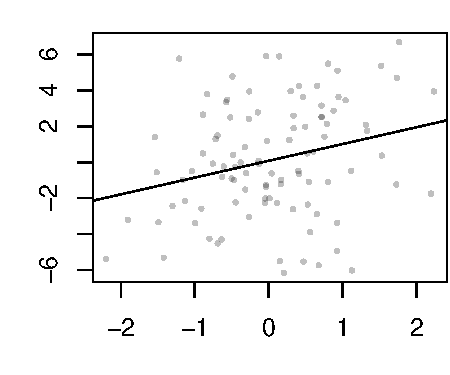
\includegraphics[height=2in]{r2ex-3.pdf}
        \[ r^2 = 0.06929872 \]
    }

\end{frame}


\section{Examples}

\section{USC weather}



%%%%%%
\begin{frame}{Back to the example}

    \begin{center}
        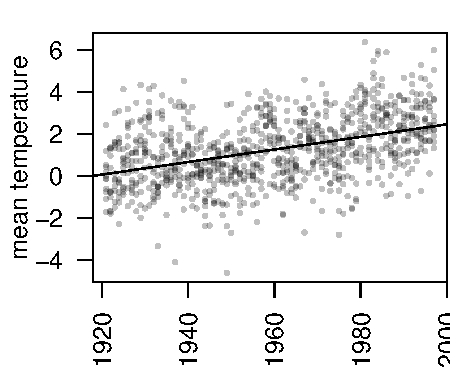
\includegraphics[height=2in]{usc-temps-just-regression}

    \begin{align*}
        r &= 0.3128291 & n &= 1114 \\
        t_s &=  r \sqrt{ \frac{ n-2}{1-r^2} } = 10.98305 &
        P &< 10^{-16} .
    \end{align*}
    What do we conclude?

    \end{center}
\end{frame}


\section{Other examples}


% . . . 

\section<article>{Summary}
\section<presentation>*{Summary}

\begin{frame}{Summary}
  \begin{enumerate}
      \item The \alert{least-squares regression line}
      \item goes through the means (center of mass)
      \item and has slope equal to the regression coefficient $r$ in normalized ($z$-score) coordinates.
      \item This line \alert{also} gives the conditional mean value of $Y$ given $X$.
      \item The residual SD measures the spread of the data about the regression line.
  \end{enumerate}
\end{frame}

% homework
\begin{frame}{Homework}
  \begin{center}

  12.2.5

  \vspace{2em}

  12.3.3

  \vspace{2em}

  12.3.6

  \end{center}
\end{frame}


\end{document}





